%% bare_jrnl_compsoc.tex
%% V1.3
%% 2007/01/11
%% by Michael Shell
%% See:
%% http://www.michaelshell.org/
%% for current contact information.
%%
%% This is a skeleton file demonstrating the use of IEEEtran.cls
%% (requires IEEEtran.cls version 1.7 or later) with an IEEE Computer
%% Society journal paper.
%%
%% Support sites:
%% http://www.michaelshell.org/tex/ieeetran/
%% http://www.ctan.org/tex-archive/macros/latex/contrib/IEEEtran/
%% and
%% http://www.ieee.org/

%%*************************************************************************
%% Legal Notice:
%% This code is offered as-is without any warranty either expressed or
%% implied; without even the implied warranty of MERCHANTABILITY or
%% FITNESS FOR A PARTICULAR PURPOSE! 
%% User assumes all risk.
%% In no event shall IEEE or any contributor to this code be liable for
%% any damages or losses, including, but not limited to, incidental,
%% consequential, or any other damages, resulting from the use or misuse
%% of any information contained here.
%%
%% All comments are the opinions of their respective authors and are not
%% necessarily endorsed by the IEEE.
%%
%% This work is distributed under the LaTeX Project Public License (LPPL)
%% ( http://www.latex-project.org/ ) version 1.3, and may be freely used,
%% distributed and modified. A copy of the LPPL, version 1.3, is included
%% in the base LaTeX documentation of all distributions of LaTeX released
%% 2003/12/01 or later.
%% Retain all contribution notices and credits.
%% ** Modified files should be clearly indicated as such, including  **
%% ** renaming them and changing author support contact information. **
%%
%% File list of work: IEEEtran.cls, IEEEtran_HOWTO.pdf, bare_adv.tex,
%%                    bare_conf.tex, bare_jrnl.tex, bare_jrnl_compsoc.tex
%%*************************************************************************

% *** Authors should verify (and, if needed, correct) their LaTeX system  ***
% *** with the testflow diagnostic prior to trusting their LaTeX platform ***
% *** with production work. IEEE's font choices can trigger bugs that do  ***
% *** not appear when using other class files.                            ***
% The testflow support page is at:
% http://www.michaelshell.org/tex/testflow/




% Note that the a4paper option is mainly intended so that authors in
% countries using A4 can easily print to A4 and see how their papers will
% look in print - the typesetting of the document will not typically be
% affected with changes in paper size (but the bottom and side margins will).
% Use the testflow package mentioned above to verify correct handling of
% both paper sizes by the user's LaTeX system.
%
% Also note that the "draftcls" or "draftclsnofoot", not "draft", option
% should be used if it is desired that the figures are to be displayed in
% draft mode.
%
% The Computer Society usually requires 10pt for submissions.
%
\documentclass[10pt,journal,letterpaper,twoside]{IEEEtran}
%
% If IEEEtran.cls has not been installed into the LaTeX system files,
% manually specify the path to it like:
% \documentclass[12pt,journal,compsoc]{../sty/IEEEtran}





% Some very useful LaTeX packages include:
% (uncomment the ones you want to load)


% *** MISC UTILITY PACKAGES ***
%
%\usepackage{ifpdf}
% Heiko Oberdiek's ifpdf.sty is very useful if you need conditional
% compilation based on whether the output is pdf or dvi.
% usage:
% \ifpdf
%   % pdf code
% \else
%   % dvi code
% \fi
% The latest version of ifpdf.sty can be obtained from:
% http://www.ctan.org/tex-archive/macros/latex/contrib/oberdiek/
% Also, note that IEEEtran.cls V1.7 and later provides a builtin
% \ifCLASSINFOpdf conditional that works the same way.
% When switching from latex to pdflatex and vice-versa, the compiler may
% have to be run twice to clear warning/error messages.






% *** CITATION PACKAGES ***
%
%\ifCLASSOPTIONcompsoc
  % IEEE Computer Society needs nocompress option
  % requires cite.sty v4.0 or later (November 2003)
  \usepackage[nocompress]{cite}
%\else
  % normal IEEE
  \usepackage{cite}
%\fi
% cite.sty was written by Donald Arseneau
% V1.6 and later of IEEEtran pre-defines the format of the cite.sty package
% \cite{} output to follow that of IEEE. Loading the cite package will
% result in citation numbers being automatically sorted and properly
% "compressed/ranged". e.g., [1], [9], [2], [7], [5], [6] without using
% cite.sty will become [1], [2], [5]--[7], [9] using cite.sty. cite.sty's
% \cite will automatically add leading space, if needed. Use cite.sty's
% noadjust option (cite.sty V3.8 and later) if you want to turn this off.
% cite.sty is already installed on most LaTeX systems. Be sure and use
% version 4.0 (2003-05-27) and later if using hyperref.sty. cite.sty does
% not currently provide for hyperlinked citations.
% The latest version can be obtained at:
% http://www.ctan.org/tex-archive/macros/latex/contrib/cite/
% The documentation is contained in the cite.sty file itself.
%
% Note that some packages require special options to format as the Computer
% Society requires. In particular, Computer Society  papers do not use
% compressed citation ranges as is done in typical IEEE papers
% (e.g., [1]-[4]). Instead, they list every citation separately in order
% (e.g., [1], [2], [3], [4]). To get the latter we need to load the cite
% package with the nocompress option which is supported by cite.sty v4.0
% and later. Note also the use of a CLASSOPTION conditional provided by
% IEEEtran.cls V1.7 and later.





% *** GRAPHICS RELATED PACKAGES ***
%
%\ifCLASSINFOpdf
%  \usepackage[pdftex]{graphicx}
  % declare the path(s) where your graphic files are
  % \graphicspath{{../pdf/}{../jpeg/}}
  % and their extensions so you won't have to specify these with
  % every instance of \includegraphics
  % \DeclareGraphicsExtensions{.pdf,.jpeg,.png}
%\else
  % or other class option (dvipsone, dvipdf, if not using dvips). graphicx
  % will default to the driver specified in the system graphics.cfg if no
  % driver is specified.
  \usepackage[dvips]{graphicx}
  % declare the path(s) where your graphic files are
  % \graphicspath{{../eps/}}
  % and their extensions so you won't have to specify these with
  % every instance of \includegraphics
  % \DeclareGraphicsExtensions{.eps}
%\fi
% graphicx was written by David Carlisle and Sebastian Rahtz. It is
% required if you want graphics, photos, etc. graphicx.sty is already
% installed on most LaTeX systems. The latest version and documentation can
% be obtained at: 
% http://www.ctan.org/tex-archive/macros/latex/required/graphics/
% Another good source of documentation is "Using Imported Graphics in
% LaTeX2e" by Keith Reckdahl which can be found as epslatex.ps or
% epslatex.pdf at: http://www.ctan.org/tex-archive/info/
%
% latex, and pdflatex in dvi mode, support graphics in encapsulated
% postscript (.eps) format. pdflatex in pdf mode supports graphics
% in .pdf, .jpeg, .png and .mps (metapost) formats. Users should ensure
% that all non-photo figures use a vector format (.eps, .pdf, .mps) and
% not a bitmapped formats (.jpeg, .png). IEEE frowns on bitmapped formats
% which can result in "jaggedy"/blurry rendering of lines and letters as
% well as large increases in file sizes.
%
% You can find documentation about the pdfTeX application at:
% http://www.tug.org/applications/pdftex





% *** MATH PACKAGES ***
%
\let\latexvec=\vec
%\usepackage[cmex10]{amsmath}
\usepackage{amssymb}
\usepackage{amsmath}
\usepackage{relsize}
\let\vec=\latexvec
% A popular package from the American Mathematical Society that provides
% many useful and powerful commands for dealing with mathematics. If using
% it, be sure to load this package with the cmex10 option to ensure that
% only type 1 fonts will utilized at all point sizes. Without this option,
% it is possible that some math symbols, particularly those within
% footnotes, will be rendered in bitmap form which will result in a
% document that can not be IEEE Xplore compliant!
%
% Also, note that the amsmath package sets \interdisplaylinepenalty to 10000
% thus preventing page breaks from occurring within multiline equations. Use:
\interdisplaylinepenalty=2500
% after loading amsmath to restore such page breaks as IEEEtran.cls normally
% does. amsmath.sty is already installed on most LaTeX systems. The latest
% version and documentation can be obtained at:
% http://www.ctan.org/tex-archive/macros/latex/required/amslatex/math/





% *** SPECIALIZED LIST PACKAGES ***
%
\usepackage{algpseudocode}
\renewcommand{\algorithmicrequire}{\textbf{Input:}}
\renewcommand{\algorithmicensure}{\textbf{Output:}}
% \usepackage{algorithmic}
% algorithmic.sty was written by Peter Williams and Rogerio Brito.
% This package provides an algorithmic environment fo describing algorithms.
% You can use the algorithmic environment in-text or within a figure
% environment to provide for a floating algorithm. Do NOT use the algorithm
% floating environment provided by algorithm.sty (by the same authors) or
% algorithm2e.sty (by Christophe Fiorio) as IEEE does not use dedicated
% algorithm float types and packages that provide these will not provide
% correct IEEE style captions. The latest version and documentation of
% algorithmic.sty can be obtained at:
% http://www.ctan.org/tex-archive/macros/latex/contrib/algorithms/
% There is also a support site at:
% http://algorithms.berlios.de/index.html
% Also of interest may be the (relatively newer and more customizable)
% algorithmicx.sty package by Szasz Janos:
% http://www.ctan.org/tex-archive/macros/latex/contrib/algorithmicx/




% *** ALIGNMENT PACKAGES ***
%
\usepackage{array}
% Frank Mittelbach's and David Carlisle's array.sty patches and improves
% the standard LaTeX2e array and tabular environments to provide better
% appearance and additional user controls. As the default LaTeX2e table
% generation code is lacking to the point of almost being broken with
% respect to the quality of the end results, all users are strongly
% advised to use an enhanced (at the very least that provided by array.sty)
% set of table tools. array.sty is already installed on most systems. The
% latest version and documentation can be obtained at:
% http://www.ctan.org/tex-archive/macros/latex/required/tools/


%\usepackage{mdwmath}
%\usepackage{mdwtab}
% Also highly recommended is Mark Wooding's extremely powerful MDW tools,
% especially mdwmath.sty and mdwtab.sty which are used to format equations
% and tables, respectively. The MDWtools set is already installed on most
% LaTeX systems. The lastest version and documentation is available at:
% http://www.ctan.org/tex-archive/macros/latex/contrib/mdwtools/


% IEEEtran contains the IEEEeqnarray family of commands that can be used to
% generate multiline equations as well as matrices, tables, etc., of high
% quality.


% \usepackage{eqparbox}
% Also of notable interest is Scott Pakin's eqparbox package for creating
% (automatically sized) equal width boxes - aka "natural width parboxes".
% Available at:
% http://www.ctan.org/tex-archive/macros/latex/contrib/eqparbox/





% *** SUBFIGURE PACKAGES ***
% \ifCLASSOPTIONcompsoc
% \usepackage[tight,normalsize,sf,SF]{subfigure}
% \else
% \usepackage[tight,footnotesize]{subfigure}
% \fi
% subfigure.sty was written by Steven Douglas Cochran. This package makes it
% easy to put subfigures in your figures. e.g., "Figure 1a and 1b". For IEEE
% work, it is a good idea to load it with the tight package option to reduce
% the amount of white space around the subfigures. Computer Society papers
% use a larger font and \sffamily font for their captions, hence the
% additional options needed under compsoc mode. subfigure.sty is already
% installed on most LaTeX systems. The latest version and documentation can
% be obtained at:
% http://www.ctan.org/tex-archive/obsolete/macros/latex/contrib/subfigure/
% subfigure.sty has been superceeded by subfig.sty.


%\ifCLASSOPTIONcompsoc
%  \usepackage[caption=false]{caption}
%  \usepackage[font=normalsize,labelfont=sf,textfont=sf]{subfig}
%\else
%  \usepackage[caption=false]{caption}
%  \usepackage[font=footnotesize]{subfig}
%\fi
% subfig.sty, also written by Steven Douglas Cochran, is the modern
% replacement for subfigure.sty. However, subfig.sty requires and
% automatically loads Axel Sommerfeldt's caption.sty which will override
% IEEEtran.cls handling of captions and this will result in nonIEEE style
% figure/table captions. To prevent this problem, be sure and preload
% caption.sty with its "caption=false" package option. This is will preserve
% IEEEtran.cls handing of captions. Version 1.3 (2005/06/28) and later 
% (recommended due to many improvements over 1.2) of subfig.sty supports
% the caption=false option directly:
%\ifCLASSOPTIONcompsoc
%  \usepackage[caption=false,font=normalsize,labelfont=sf,textfont=sf]{subfig}
%\else
  \usepackage[caption=false,font=footnotesize]{subfig}
%\fi
%
% The latest version and documentation can be obtained at:
% http://www.ctan.org/tex-archive/macros/latex/contrib/subfig/
% The latest version and documentation of caption.sty can be obtained at:
% http://www.ctan.org/tex-archive/macros/latex/contrib/caption/




% *** FLOAT PACKAGES ***
%
\usepackage{fixltx2e}
% fixltx2e, the successor to the earlier fix2col.sty, was written by
% Frank Mittelbach and David Carlisle. This package corrects a few problems
% in the LaTeX2e kernel, the most notable of which is that in current
% LaTeX2e releases, the ordering of single and double column floats is not
% guaranteed to be preserved. Thus, an unpatched LaTeX2e can allow a
% single column figure to be placed prior to an earlier double column
% figure. The latest version and documentation can be found at:
% http://www.ctan.org/tex-archive/macros/latex/base/
\usepackage{float}


%\usepackage{stfloats}
% stfloats.sty was written by Sigitas Tolusis. This package gives LaTeX2e
% the ability to do double column floats at the bottom of the page as well
% as the top. (e.g., "\begin{figure*}[!b]" is not normally possible in
% LaTeX2e). It also provides a command:
%\fnbelowfloat
% to enable the placement of footnotes below bottom floats (the standard
% LaTeX2e kernel puts them above bottom floats). This is an invasive package
% which rewrites many portions of the LaTeX2e float routines. It may not work
% with other packages that modify the LaTeX2e float routines. The latest
% version and documentation can be obtained at:
% http://www.ctan.org/tex-archive/macros/latex/contrib/sttools/
% Documentation is contained in the stfloats.sty comments as well as in the
% presfull.pdf file. Do not use the stfloats baselinefloat ability as IEEE
% does not allow \baselineskip to stretch. Authors submitting work to the
% IEEE should note that IEEE rarely uses double column equations and
% that authors should try to avoid such use. Do not be tempted to use the
% cuted.sty or midfloat.sty packages (also by Sigitas Tolusis) as IEEE does
% not format its papers in such ways.




%\ifCLASSOPTIONcaptionsoff
%  \usepackage[nomarkers]{endfloat}
% \let\MYoriglatexcaption\caption
% \renewcommand{\caption}[2][\relax]{\MYoriglatexcaption[#2]{#2}}
%\fi
% endfloat.sty was written by James Darrell McCauley and Jeff Goldberg.
% This package may be useful when used in conjunction with IEEEtran.cls'
% captionsoff option. Some IEEE journals/societies require that submissions
% have lists of figures/tables at the end of the paper and that
% figures/tables without any captions are placed on a page by themselves at
% the end of the document. If needed, the draftcls IEEEtran class option or
% \CLASSINPUTbaselinestretch interface can be used to increase the line
% spacing as well. Be sure and use the nomarkers option of endfloat to
% prevent endfloat from "marking" where the figures would have been placed
% in the text. The two hack lines of code above are a slight modification of
% that suggested by in the endfloat docs (section 8.3.1) to ensure that
% the full captions always appear in the list of figures/tables - even if
% the user used the short optional argument of \caption[]{}.
% IEEE papers do not typically make use of \caption[]'s optional argument,
% so this should not be an issue. A similar trick can be used to disable
% captions of packages such as subfig.sty that lack options to turn off
% the subcaptions:
% For subfig.sty:
% \let\MYorigsubfloat\subfloat
% \renewcommand{\subfloat}[2][\relax]{\MYorigsubfloat[]{#2}}
% For subfigure.sty:
% \let\MYorigsubfigure\subfigure
% \renewcommand{\subfigure}[2][\relax]{\MYorigsubfigure[]{#2}}
% However, the above trick will not work if both optional arguments of
% the \subfloat/subfig command are used. Furthermore, there needs to be a
% description of each subfigure *somewhere* and endfloat does not add
% subfigure captions to its list of figures. Thus, the best approach is to
% avoid the use of subfigure captions (many IEEE journals avoid them anyway)
% and instead reference/explain all the subfigures within the main caption.
% The latest version of endfloat.sty and its documentation can obtained at:
% http://www.ctan.org/tex-archive/macros/latex/contrib/endfloat/
%
% The IEEEtran \ifCLASSOPTIONcaptionsoff conditional can also be used
% later in the document, say, to conditionally put the References on a 
% page by themselves.




% *** PDF, URL AND HYPERLINK PACKAGES ***
%
\usepackage{url}
% url.sty was written by Donald Arseneau. It provides better support for
% handling and breaking URLs. url.sty is already installed on most LaTeX
% systems. The latest version can be obtained at:
% http://www.ctan.org/tex-archive/macros/latex/contrib/misc/
% Read the url.sty source comments for usage information. Basically,
% \url{my_url_here}.


% Other packages
\usepackage{becs}

\usepackage{listings}
\lstset{%
  basicstyle=\scriptsize,
  numbers=left,
  numberstyle=\tiny,
  stepnumber=1,
  xleftmargin=2em
}

% Theorem-like environments
\newtheorem{definition}{Definition}
\newtheorem{exampleb}{Example}

% \subsubsubsection - really!?
\newcommand{\subsubsubsection}[1]{\medskip\par\emph{#1:}}

% *** Do not adjust lengths that control margins, column widths, etc. ***
% *** Do not use packages that alter fonts (such as pslatex).         ***
% There should be no need to do such things with IEEEtran.cls V1.6 and later.
% (Unless specifically asked to do so by the journal or conference you plan
% to submit to, of course. )


% correct bad hyphenation here
\hyphenation{op-tical net-works semi-conduc-tor}
\usepackage{color}
%\usepackage{subfigure}

\begin{document}
%
% paper title
% can use linebreaks \\ within to get better formatting as desired
\title{An improved metric for the analysis of swarms}
%
%
% author names and IEEE memberships
% note positions of commas and nonbreaking spaces ( ~ ) LaTeX will not break
% a structure at a ~ so this keeps an author's name from being broken across
% two lines.
% use \thanks{} to gain access to the first footnote area
% a separate \thanks must be used for each paragraph as LaTeX2e's \thanks
% was not built to handle multiple paragraphs
%
%
%\IEEEcompsocitemizethanks is a special \thanks that produces the bulleted
% lists the Computer Society journals use for "first footnote" author
% affiliations. Use \IEEEcompsocthanksitem which works much like \item
% for each affiliation group. When not in compsoc mode,
% \IEEEcompsocitemizethanks becomes like \thanks and
% \IEEEcompsocthanksitem becomes a line break with idention. This
% facilitates dual compilation, although admittedly the differences in the
% desired content of \author between the different types of papers makes a
% one-size-fits-all approach a daunting prospect. For instance, compsoc 
% journal papers have the author affiliations above the "Manuscript
% received ..."  text while in non-compsoc journals this is reversed. Sigh.

\author{Neil Eliot, David Kendall, Michael Brockway
\IEEEcompsocitemizethanks{\IEEEcompsocthanksitem
N.~Eliot
D.~Kendall
M.~Brockway are from Northumbria University, UK}
\thanks{}}

% note the % following the last \IEEEmembership and also \thanks - 
% these prevent an unwanted space from occurring between the last author name
% and the end of the author line. i.e., if you had this:
% 
% \author{....lastname \thanks{...} \thanks{...} }
%                     ^------------^------------^----Do not want these spaces!
%
% a space would be appended to the last name and could cause every name on that
% line to be shifted left slightly. This is one of those "LaTeX things". For
% instance, "\textbf{A} \textbf{B}" will typeset as "A B" not "AB". To get
% "AB" then you have to do: "\textbf{A}\textbf{B}"
% \thanks is no different in this regard, so shield the last } of each \thanks
% that ends a line with a % and do not let a space in before the next \thanks.
% Spaces after \IEEEmembership other than the last one are OK (and needed) as
% you are supposed to have spaces between the names. For what it is worth,
% this is a minor point as most people would not even notice if the said evil
% space somehow managed to creep in.



% The paper headers
\markboth{IEEE Transactions on Automatic Control}%
{N.~Eliot: An improved metric for the analysis of swarms}
% The only time the second header will appear is for the odd numbered pages
% after the title page when using the twoside option.
% 
% *** Note that you probably will NOT want to include the author's ***
% *** name in the headers of peer review papers.                   ***
% You can use \ifCLASSOPTIONpeerreview for conditional compilation here if
% you desire.



% The publisher's ID mark at the bottom of the page is less important with
% Computer Society journal papers as those publications place the marks
% outside of the main text columns and, therefore, unlike regular IEEE
% journals, the available text space is not reduced by their presence.
% If you want to put a publisher's ID mark on the page you can do it like
% this:
%\IEEEpubid{0000--0000/00\$00.00~\copyright~2007 IEEE}
% or like this to get the Computer Society new two part style.
%\IEEEpubid{\makebox[\columnwidth]{\hfill 0000--0000/00/\$00.00~\copyright~2007 IEEE}%
%\hspace{\columnsep}\makebox[\columnwidth]{Published by the IEEE Computer Society\hfill}}
% Remember, if you use this you must call \IEEEpubidadjcol in the second
% column for its text to clear the IEEEpubid mark (Computer Society jorunal
% papers don't need this extra clearance.)




% for Computer Society papers, we must declare the abstract and index terms
% PRIOR to the title within the \IEEEcompsoctitleabstractindextext IEEEtran
% command as these need to go into the title area created by \maketitle.
\IEEEcompsoctitleabstractindextext{%
\begin{abstract}
%\boldmath
An important criteria in the application of swarm coordination algorithms is the extent to which they cause unnecessary movement. i.e. movement which occurs as a side affect of the algorithm rather than the the intended function. This paper examines the widely used distance metric as a mechanism to measure the internal movement of agents and introduces a new \textit{magnitude based metric}. 

Both metrics are based upon the resultant internal movement of a swarm identified by analysing the changes in the inter-agent interactions. The two metrics differ in their approach to identifying the changes. The distance metric uses variations in the inter-agent distances and the new metric uses the resultant magnitudes from the agents' \textit{inter-agent vector magnitudes}  which we claim offers a number of advantages over the distance metric. 

Both metrics allow a comparison of the effects of different swarming algorithms on a swarm's structure to identify the `level' of change in a swarm's internal structure which is an indication of the amount of unnecessary movement an algorithm creates. 

In addition the magnitude based metric also identifies a swarm as expanding or cohesive.
This additional information has practical benefits for the implementation of algorithms for hetrogenious swarms.

\end{abstract}
% IEEEtran.cls defaults to using nonbold math in the Abstract.
% This preserves the distinction between vectors and scalars. However,
% if the journal you are submitting to favors bold math in the abstract,
% then you can use LaTeX's standard command \boldmath at the very start
% of the abstract to achieve this. Many IEEE journals frown on math
% in the abstract anyway. In particular, the Computer Society does
% not want either math or citations to appear in the abstract.

% Note that keywords are not normally used for peer review papers.
\begin{IEEEkeywords}
Swarming, Swarm Dynamics, Mobile Sensor Networks, Algorithms.
\end{IEEEkeywords}}


% make the title area
\maketitle


% To allow for easy dual compilation without having to reenter the
% abstract/keywords data, the \IEEEcompsoctitleabstractindextext text will
% not be used in maketitle, but will appear (i.e., to be "transported")
% here as \IEEEdisplaynotcompsoctitleabstractindextext when compsoc mode
% is not selected <OR> if conference mode is selected - because compsoc
% conference papers position the abstract like regular (non-compsoc)
% papers do!
\IEEEdisplaynotcompsoctitleabstractindextext
% \IEEEdisplaynotcompsoctitleabstractindextext has no effect when using
% compsoc under a non-conference mode.


% For peer review papers, you can put extra information on the cover
% page as needed:
% \ifCLASSOPTIONpeerreview
% \begin{center} \bfseries EDICS Category: 3-BBND \end{center}
% \fi
%
% For peerreview papers, this IEEEtran command inserts a page break and
% creates the second title. It will be ignored for other modes.
\IEEEpeerreviewmaketitle


\section{Introduction\label{sec:intro}}

%\section{Introduction\label{methods:SwarmStability}}
\emph{Swarming} in the animal kingdom of ants, bees, fish and birds for instance has long been studied by scientists. From these studies mathematical models and algorithms have evolved. The models and algorithms have in turn captured the interest of computing scientists who are interested in applying them to large groups of autonomous mobile \emph{agents} (`robots'). The cooperative coordination of these agents can take many forms such as following a set path~\cite{HCS:09}, existing in a static space~\cite{EP:10, GP:02, GP:04} or foraging as a colony~\cite{HER:11, GK:07}. One of the attributes of swarms that has captured the interest of scientists is that the models and algorithms used to coordinate them are generally sets of simple rules. These simple rules cause the agents to appear to work cooperatively. These rules can also generate movement that does not contribute to the goal of the swarm this movement is a direct result of the agents attempting to move towards an optimum position within the structure. This internal movement can be identified by analysing the changes in the inter-agent interactions. Measuring this unnecessary movement allows the effectivemness of a swarming algorithm to be evaluated. If the internal movement can be reduced then stability of the swarm is improved and more of the swarms energy is focused on the goal. Also reducing the internal movement also provides a more stable platform for the deployment of sensor arrays. Both metric allow this evaluation to be caried out when all the sensor ranges are the same however the distance metric is not able to identify the internal movement accurately when the sensor ranges of each agent varies producing varyig distances even though the interactions at the magnitude level indicates the agents are in fact stable and optimum. This paper discusses two metrics and how they differ in their approach to identify these changes. The distance metric uses variations in the inter-agent spaces, as used by Navarro et al.~\cite{NIM:09}. The new metric uses the resultant magnitudes from an agents' \textit{inter-agent vectors} that are induced by an agent interacting with its neighbours which allows a more acurate analysis of a swarm when using non homogenous sensor distances The metric also identifies when a swarm is expanding or contracting. 

This paper presents a swarm model and then applies the two metrics to this model to present a comparison of the two metrics and uses the new metric to identify a swarm's `state'.
 
%% \section{Metric principles\label{section:MagnitudeDynamics}}
%% This section discusses the theory behind swarm movement and the effects that can be measured using both the metrics described above.
\section{Swarm modelling}\label{SwarmModelling}
Currently, much swarm research uses field effects as the method of modelling inter-agent interactions~\cite{BAF:06, BAFVM:06, BM:09, APZDAMC:09, GP:02, GP:04, GP:04a, GP:05, GP:11, MYP:09}. The models usually use two field effects to implement the swarming characteristic. These effects are \textit{cohesion}, to draw agents closer, and \textit{repulsion} to prevent agents colliding. Field effects are the ranges around an agent that determine the effect other agents have upon its movement~(Figure~\ref{methods:FieldEffects}). It is usual for the cohesion field to have a radius $C_b$ which is larger than the repulsion radius $R_b$. When an agent ($b'$) moves into the \textit{neighbour field} of an agent ($b$) then $b'$ is said to be a neighbour of $b$ and is subject to cohesion. When an agent $b'$ moves into the repulsion field of $b$ then $b$ has a tendency to move away from $b'$, i.e. to be repulsed. When an agent $b$ moves too close to an obstacle, i.e. within the obstacle repulsion range $O_b$, it has a tendency to move away from the obstacle.

\begin{figure}[H]
\begin{center}
\includegraphics[width=6cm]{figures/FieldEffects}
\end{center}
\caption{Agent field effects\label{methods:FieldEffects}}
\end{figure}

\section{Inter-agent vector magnitude effect on internal movement}\label{Section:StabilityMagnitude}
Figure \ref{methods:Stability5} shows the cohesion and repulsion vector contributions to $v_c(b)$ and $v_r(b)$ due to neighbour $b'$, as given in (Equations \ref{eq:FlyToCentre1} and \ref{eq:Repulsion1}). Notice that the vectors are along the line of separation $bb'$. \\

%% Equation (\ref{eq:Neighbours1}) identifies the set of agents that are neigbours of $b$.
%% 
%% \begin{equation}\label{eq:Neighbours1}
%% nbr(b) \buildrel \Delta \over = \{b' \in S | |bb'| <= C_b\}
%% \end{equation}‎

Equation (\ref{eq:FlyToCentre1}) identifies the resultant cohesion effect of all the neighbours of $b$. $nbr(.)$ returns a set of all the agents in the swarm that are a neighbour of $b$. A neighbour is any agent that fails within the cohesion field.

\begin{equation}\label{eq:FlyToCentre1}
v_{c}(b) = \frac{1}{|nbr(b)|}\left({\mathlarger{\sum_{b' \in nbr(b)}}{bb'}}\right)
\end{equation}‎

Equation (\ref{eq:Repulsion1}) identifies the resultant repulsion effect of all the neighbours of $b$ where $rep(.)$ returns a set of all agents that are within the repulsion field.

\begin{equation}
\label{eq:Repulsion1}
v_{r}(b) =‎ -
\frac{1}{|rep(b)|}
\left(
\mathlarger{\mathlarger{\sum_{b' \in rep(b)}}}
{\left( 1-\frac{|bb'|}{R_b} \right)}
{bb'}
\right)
\end{equation}‎

Using the cohesion and repulsion vectors generated by the relationship of $b$ to its neighbour a resultant vector can be calculated. This vector creates an agent characteristic that can be used as a metric. Summing the vectors creates a resultant vector with a magnitude that affects the agent. Summing the vectors also provides an indication of the direction an agent will move based on the relationship. This is the \textit{inter-agent vector}.

Equation (\ref{eq:InterAgentMovement1}) identifies the \textit{inter-agent vector} for agent $b$ with respect to its neighbours.

\begin{equation}\label{eq:InterAgentMovement1}
v(b) = v_{c}(b) + v_{r}(b)
\end{equation}‎

If a weighted model is used then equation~\ref{eq:InterAgentMovement1} becomes equation~\ref{eq:InterAgentMovement2}.

\begin{equation}\label{eq:InterAgentMovement2}
v(b) = k_cv_{c}(b) + k_rv_{r}(b)
\end{equation}‎

where $k_c$ and $k_r$ are weightings to change the effect of each vector as shown in Table~\ref{tab:MetricPhysics1}.

%% From here throughout sections \ref{metric:MagnitudeDynamics2} and \ref{metric:StabilityNullVector} imagine agent $b$ has just a single neighbour $b'$ and consider the effect of $b'$ on $v(b)$, the \textit{inter-agent vector} of $b$.
%% The relationship between the agents is that: \emph{the vector for $b$ with respect to $b^{'}$, and the vector for $b^{'}$ with respect to $b$ are on the same line}~(\ref{methods:Stability5}).
%% If we consider an agent ($b$) as having only one neighbour ($b'$) then using the formulae defined in chapter~\ref{chapter:methods} the vectors $v_c(b)$~(\ref{eq:FlyToCentre1}) and $v_r(b)$~(\ref{eq:Repulsion1}) are the magnitudes of the vectors that are generated by the field effects between the two agents. $k_c$ and $k_r$ are the weighting factors for the cohesion and repulsion. The resulting vectors are aligned along the same line of separation between the agents. 

\begin{figure}[H]
\begin{center}
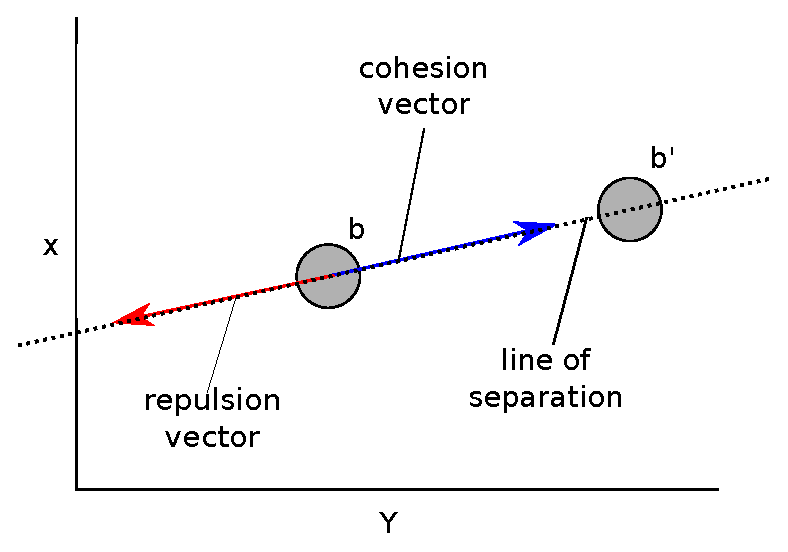
\includegraphics[width=7cm]{figures/Stability5}
\end{center}
\caption{Vectors on line of separation} \label{methods:Stability5}
\end{figure}

\section{Swarm movement analysis\label{metric:MagnitudeDynamics2}}
The repulsion and cohesion vectors are generated for an agent through the interaction of their field effects~(Figure~\ref{methods:FieldEffects}). There are a limited number of interactions that can occur; These are illustrated in Figures \ref{methods:Stability1}, \ref{methods:Stability2}, \ref{methods:Stability3} and \ref{methods:Stability4}.

Following repeated experments in the initial deployment of a swarm it was found that using the same parameters for a swarm's environmental parameters and the cohesion and repulsion ranges that the results where always very similar. The results shown in this paper are therefore an example set typical of the results obtained. The data extracts shown in Tables \ref{tab:SampleReplusion0}, \ref{tab:SampleReplusionPositive}, \ref{tab:SampleCohesionPositive} and  \ref{tab:SampleEquilibrium}) show the simulation results that are produced by the parameters listed in Table~\ref{tab:MetricPhysics1}. The simulation consists of 200 agents over a 20 second period. The cohesion of an agent pair is shown as $k_cv_c$ and the repulsion as $k_rv_r$.

\begin{table}[H]
\begin{center}
\begin{tabular}{| p{2.5cm} | c | p{3cm} |}
\hline
\bf Weight \bf Component & \bf Setting & \bf Description \\ \hline
Sample Rate & 100 & ms - Unit sampling interval\\  \hline
$k_c$ & 5 & weight adjuster for cohesion bias\\  \hline
$k_r$ & 15 & weight adjuster for repulsion  bias\\  \hline
$k_d$ & 0 & weight adjuster for directional bias 0 for static baseline 100 from directional\\  \hline
Repulsion Boundary & 70 & units\\  \hline
Neighbour Distance & 80 & units\\  \hline
Speed & 20 & units/s\\  \hline
\end{tabular}\caption{Swarm model parameters} \label{tab:MetricPhysics1}
\end{center}
\end{table}

Figure~\ref{methods:Stability1} shows two agents within each other's cohesion fields but sufficiently distant to be outside of the repulsion fields. In this case $|k_cv_c| > 0$ and $|k_rv_r| = 0$: the result is the agent's resultant magnitude $v(b$  cause the agent to move towards is neighbour $b'$. Likewise the neighbours resultant magnitude $v(b')$ will cause the agent to move towards $b$. Table~\ref{tab:SampleReplusion0} shows the repulsion magnitude with a value of 0. The only influence on the agent pairs are cohesive vectors. 

\begin{figure}[H]
\begin{center}
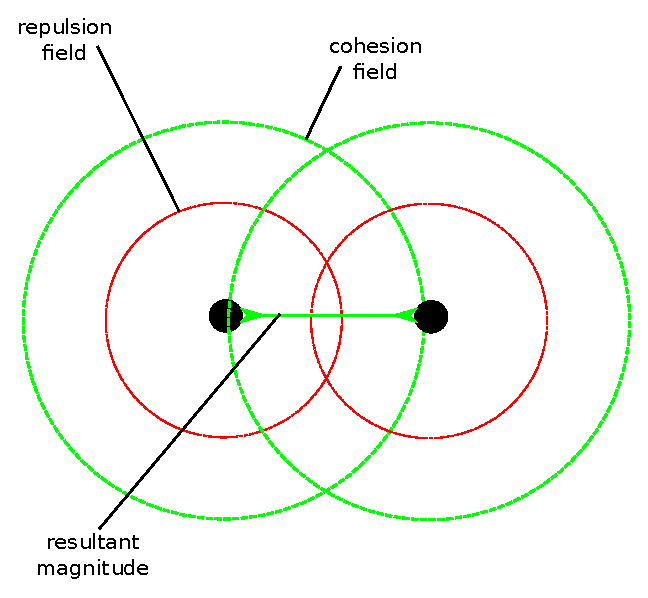
\includegraphics[width=6cm]{figures/Stability1}
\end{center}
\caption{Internal movement cohesion (no repulsion)} \label{methods:Stability1}
\end{figure}

\begin{table}[H]
\begin{center}
\begin{tabular}{| l | l | l | l | l | l |}
\hline
Log &	Id &	N.Id &	Distance &	{\color{green}Cohesion} &	{\color{red}Repulsion} 	\\ \hline
0 &	1 &	3 	 & 70.50359 &	{\color{green}352.51799} &	{\color{red}0} \\ \hline
0 &	1 &	100 & 71.78005 &	{\color{green}358.90027} &	{\color{red}0} \\ \hline
0 &	1 &	151 & 78.33995 &	{\color{green}391.69979} &	{\color{red}0} \\ \hline
0 &	2 &	99  &	72.04066 &	{\color{green}360.20334} &	{\color{red}0} \\ 
\hline
\end{tabular}\caption{Data extract ($|k_rv_r| = 0$)} \label{tab:SampleReplusion0}
\end{center}
\end{table}

Figure~\ref{methods:Stability2} shows two agents close together with repulsion dominating cohesion such that $|k_cv_c|~<~|k_rv_r|$. The resultant vector direct the agents away from each other. 

Table~\ref{tab:SampleReplusionPositive} shows the repulsion magnitude with a value greater than cohesion.

\begin{figure}[H]
\begin{center}
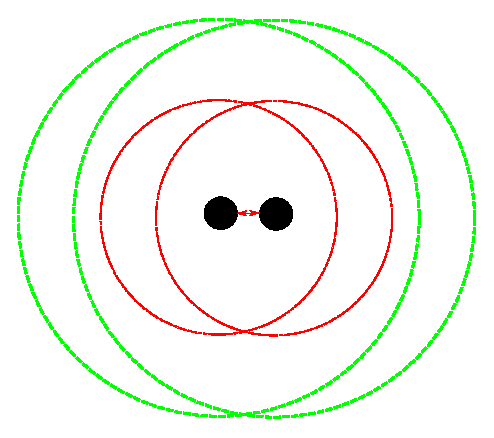
\includegraphics[width=6cm]{figures/Stability2}
\end{center}
\caption{Internal movement repulsion} \label{methods:Stability2}
\end{figure}

\begin{table}[H]
\begin{center}
\begin{tabular}{| l | l | l | l | l | l |}
\hline
Log &	Id &	N.Id &	Distance &	{\color{green}Cohesion} &	{\color{red}Repulsion} 	\\ \hline
0 & 1 & 2 & 28.32522 & {\color{green}141.62612} & {\color{red}1544.86014} \\ \hline
0 & 1 & 6 & 41.48517 & {\color{green}207.42586} & {\color{red}721.71736} \\ \hline
0 & 1 & 7 & 35.26412 & {\color{green}176.32064} & {\color{red}1034.27101} \\ \hline
0 & 1 & 8 & 43.54503 & {\color{green}217.72518} & {\color{red}637.90759} \\
\hline
\end{tabular}\caption{Data extract ($|k_cv_c| < |k_rv_r|$)} \label{tab:SampleReplusionPositive}
\end{center}
\end{table}

Figure~\ref{methods:Stability3} shows two agents close together but with cohesion vector magnitudes greater than the repulsion magnitudes $|k_cv_c|~>~|k_rv_r|$. The resultant vector draws the agents together. The magnitude of the resultant cohesion vector reduces due to the cancelling effect of the repulsion vector. Table~\ref{tab:SampleCohesionPositive} shows a data extract with the cohesion magnitude greater than repulsion.

\begin{figure}[H]
\begin{center}
\includegraphics[width=6cm]{figures/Stability3}
\end{center}
\caption{Internal movement cohesion and repulsion} \label{methods:Stability3}
\end{figure}

\begin{table}[H]
\begin{center}
\begin{tabular}{| l | l | l | l | l | l |}
\hline
Log &	Id &	N.Id &	Distance &	{\color{green}Cohesion} & {\color{red}Repulsion} 	\\ \hline
0 & 1 & 5 &	64.17214 &	{\color{green}320.86072} &	{\color{red}95.35676} \\ \hline
0 & 1 & 9 &	63.88049 &	{\color{green}319.40248} &	{\color{red}100.58590} \\ \hline
0 & 1 & 95 & 65.61522 &	{\color{green}328.07613} &	{\color{red}70.16681} \\ \hline
0 & 1 & 152 & 63.10700 & {\color{green}315.5350} & {\color{red}114.68844} \\ 
\hline
\end{tabular}\caption{Data extract ($|k_cv_c| > |k_rv_r|$)} \label{tab:SampleCohesionPositive}
\end{center}
\end{table}

Figure~\ref{methods:Stability4} shows two agents close together with $|k_cv_c|~=~|k_rv_r|$ the resultant vector is a \textit{null vector} and the agents have no influence upon each other due to the magnitude of the resultant vector being zero. Table~\ref{tab:SampleEquilibrium} is an extract of data from the simulator. The data shows near equilibrium but due to the dynamic nature of a swarm system no agents meet the condition fully. 

\begin{figure}[H]
\begin{center}
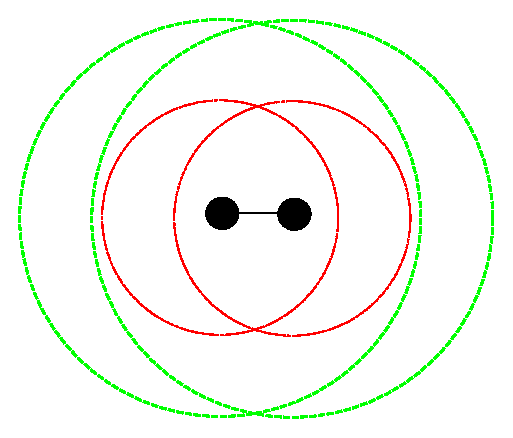
\includegraphics[width=6cm]{figures/Stability4}
\end{center}
\caption{Internal movement equilibrium} \label{methods:Stability4}
\end{figure}

\begin{table}[H]
\begin{center}
\begin{tabular}{| l | l | l | l | l | l |}
\hline
Log &	Id &	N.Id &	Distance &	{\color{green}Cohesion} &	{\color{red}Repulsion} 	\\ \hline
7 & 76 &	91 & 55.39031 & {\color{green}276.95156} & {\color{red}276.94684} \\ \hline
24 & 75 & 6 & 55.39032 & {\color{green}276.95160} & {\color{red}276.94661} \\ \hline
32 & 72 & 38 &	55.39002603773678 & {\color{green}276.95013} & {\color{red}276.95370} \\ \hline
35 &	63 & 64 & 55.39022 &	{\color{green}276.95113} &	{\color{red}276.94887} \\
\hline
\end{tabular}\caption{Data extract ($|k_cv_c| \approx |k_rv_r|$)} \label{tab:SampleEquilibrium}
\end{center}
\end{table}

\section{Internal movement and the null vector}\label{metric:StabilityNullVector}
When the two vectors (cohesion and repulsion) have magnitudes that are equal and opposite they produce a null vector. This indicates that two agents are optimally spaced for a given set of conditions. Although the agents are at an optimum position it does not mean the swarm is optimally distributed. If a swarm is in a confined space it is possible for an optimum position to be created where the vector magnitude is affected by a compression effect. This phenomenon is used in the identification of the emergent behaviour of \textit{area flooding}.  

If we consider the equilibrium state (Figure~\ref{methods:Stability4}) the resultant vector of $b$ is $(0,0)$. A null vector cannot be normalised to produce a directional vector ($\hat{v} = \frac{v}{|v|}$ if $v\neq0$; $0$ if $v=0$) The effect of the resultant magnitude being a null vector is that the agent will remain stationary. If all agent pairs are in this condition the swarm will stop moving~(Figure~\ref{methods:StabilityNullVector}).

\begin{figure}[H]
\begin{center}
\includegraphics[width=6cm]{figures/StabilityNullVector}
\end{center}
\caption{Equilibrium with null vectors} \label{methods:StabilityNullVector}
\end{figure}

Due to $v(b)$ the independent nature of the agents this situation is very rare. The residual motion that persists in a swarm is the background `noise' or `jitter' that an algorithm creates.

If a swarm is goal-based the addition of a \textit{directional vector} will prevent all agents simultaneously producing null vectors~(Figure~\ref{concave:VoidPerimeter2}, Equation~\ref{eq:InterAgentMovementDirectional1}). Where $k_dv_{d}(b)$ is the calculated directional vector to be applied to an agent.

\begin{equation}\label{eq:InterAgentMovementDirectional1}
v(b) = k_cv_{c}(b) + k_rv_{r}(b) + k_dv_{d}(b)
\end{equation}‎

\begin{figure}[H]
\begin{center}
	 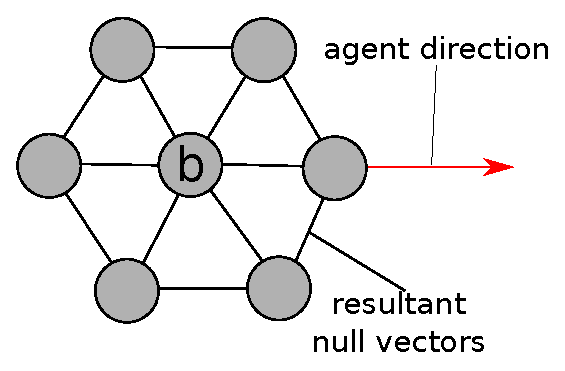
\includegraphics[width=5.5cm]{figures/StabilityNullVector3}
\end{center}
\label{concave:VoidPerimeter1}
\caption{(t)}
\end{figure}

\begin{figure}[H]
\begin{center}
	 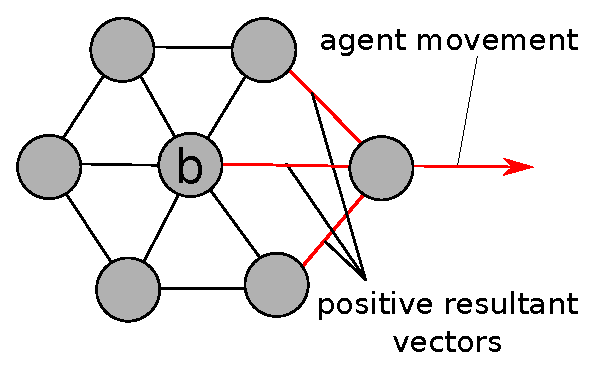
\includegraphics[width=6cm]{figures/StabilityNullVector2}
\end{center}
\caption{(t + 1)}
\label{concave:VoidPerimeter2}
\end{figure}

\section{Residual internal movement (Jitter)}\label{metric:Jitter}
Due to the dynamic nature of a swarm, maintaining optimum internal movement as in~Figure \ref{methods:StabilityNullVector} is highly unlikely. The agent pairs may fluctuate between the 4 states~(Figures~\ref{methods:Stability1}, \ref{methods:Stability2}, \ref{methods:Stability3} and \ref{methods:Stability4}). This transitions are \textit{jitter}. The degree to which this variation occurs can be measured using either the change in distance between the agents, or the change in the magnitude $P(b)$ (Equation~\ref{eq:BotStabilityT}) between the agents. Jitter arises as motion to maintain the structure of a swarm. A swarm coordination algorithm that reduces jitter is generally desirable. 

\section{Distance based metric\label{section:DistanceDynamics}}
The distance-based metric considers a swarm in terms of how the agents are physically distributed: i.e. only the inter-agent distances and their standard deviation are considered. The standard deviation indicates the extent to which the swarm is out of balance and will move to re-balance itself. If the standard deviation is zero then all the agents are evenly spaced. 

%The distance metric does not take into consideration the vector magnitudes between the agents as discussed above. The metric therefore is unable to identify the potential state of the swarm in terms of its cohesive or repulsive state.

Navarro and Fernando describe a \textit{mean distance error} metric that is based on the variations in distances between inter-agent spaces~\cite{NIM:09}. This is the same as the standard deviation of the distance based internal movement metric. 


%% \section{Distance metric internal movement}
%% The distance based internal movement is measured by identifying the mean length of the vectors between an agent and its neighbours. As with the \textit{agent resultant magnitude} a coordination algorithm produces `jitter' which is the variations from the mean. In the case of the distance based metric the jitter is identified by the changes in the distances rather than the changes in vector magnitude (\textit{agent resultant magnitude}). The distance metric is the mean and the standard deviation `jitter' of the inter-agent distances.

\section{Calculating distance based internal movement}
Equation~\ref{eq:SwarmStabilityDistance1} computes the means distance of an agent to its neighbours $nbr(b)$. 
%% The relative position vector generated for an agent $b$ to its neighbour $b'$, $bb'$, is shown in~(\ref{eq:FlyToCentre1}). The magnitude of that vector gives the distance between two agents. For an individual agent the average magnitude $\mu_d(b)$ is calculated as \ref{eq:SwarmStabilityDistance1} where $b$ is the agent and $|nbr(b)|$ is the number of neighbours.

\begin{equation}
\label{eq:SwarmStabilityDistance1}
\mu_d(b) = \frac{1}{\mathlarger{|nbr(b)|}}\left({\mathlarger{\sum_{b' \in nbr(b)}}|bb'|}\right)
\end{equation}

The mean distance for a swarm is calculated by Equation~\ref{eq:SwarmStabilityDistance2}. All the inter-agent distances are included for the swarm ($S$). 

%% $\sum_{b \in S}|nbr(b)|$ calculates how many inter-agent relationships exist in the swarm and $\sum_{b' \in nbr(b)}|bb'|$ calculates the total distance between each agent and its neighbours. $\sum_{b \in S}$ iterates over all the agents in the swarm~($S$).

\begin{equation}
\label{eq:SwarmStabilityDistance2}
\mu_d(S) = \frac{\mathlarger{\sum_{b \in S}}~\mathlarger{\sum_{b' \in nbr(b)}}|bb'|}{\mathlarger{\sum_{b \in S}|nbr(b)|}}
\end{equation}

\section{Standard deviation in distance metric}\label{Section:VarianceInDistance}
The mechanism above provides an overall indication of the distribution of the agents. The model for a swarm $S$ ($\mu_d(S)$) is not sufficient to give an indication of the internal distribution of the agents. The standard deviation clarifies the distribution within the swarm as shown in~Equation~\ref{eq:SwarmStabilityDistance3}. 

%% $(|bb'| - \mu(S))^2$ is the square of the difference in a distance to the mean and $\sum_{b \in S}~\sum_{b' \in nbr(b)}$ calculates the number of inter-agent interactions.

\begin{equation}
\label{eq:SwarmStabilityDistance3}
\sigma_d(S) = \sqrt{\frac{\mathlarger{\sum_{b \in S}}~\mathlarger{\sum_{b' \in nbr(b)}}\Big(|bb'| - \mu_d(S)\Big)^2}{\mathlarger{\sum_{b \in S}|nbr(b)|}}}
\end{equation}

The distance metric for the internal distribution of the agents is the pair consisting of $\mu_d(S)$, $\sigma_d(S)$. This can be written informally as:

\begin{equation}
\label{eq:SwarmPotentialMagnitude}
\psi_d(S) = \mu_d(S)\pm \sigma_d(S)
\end{equation}

\begin{figure}[H]
\begin{center}
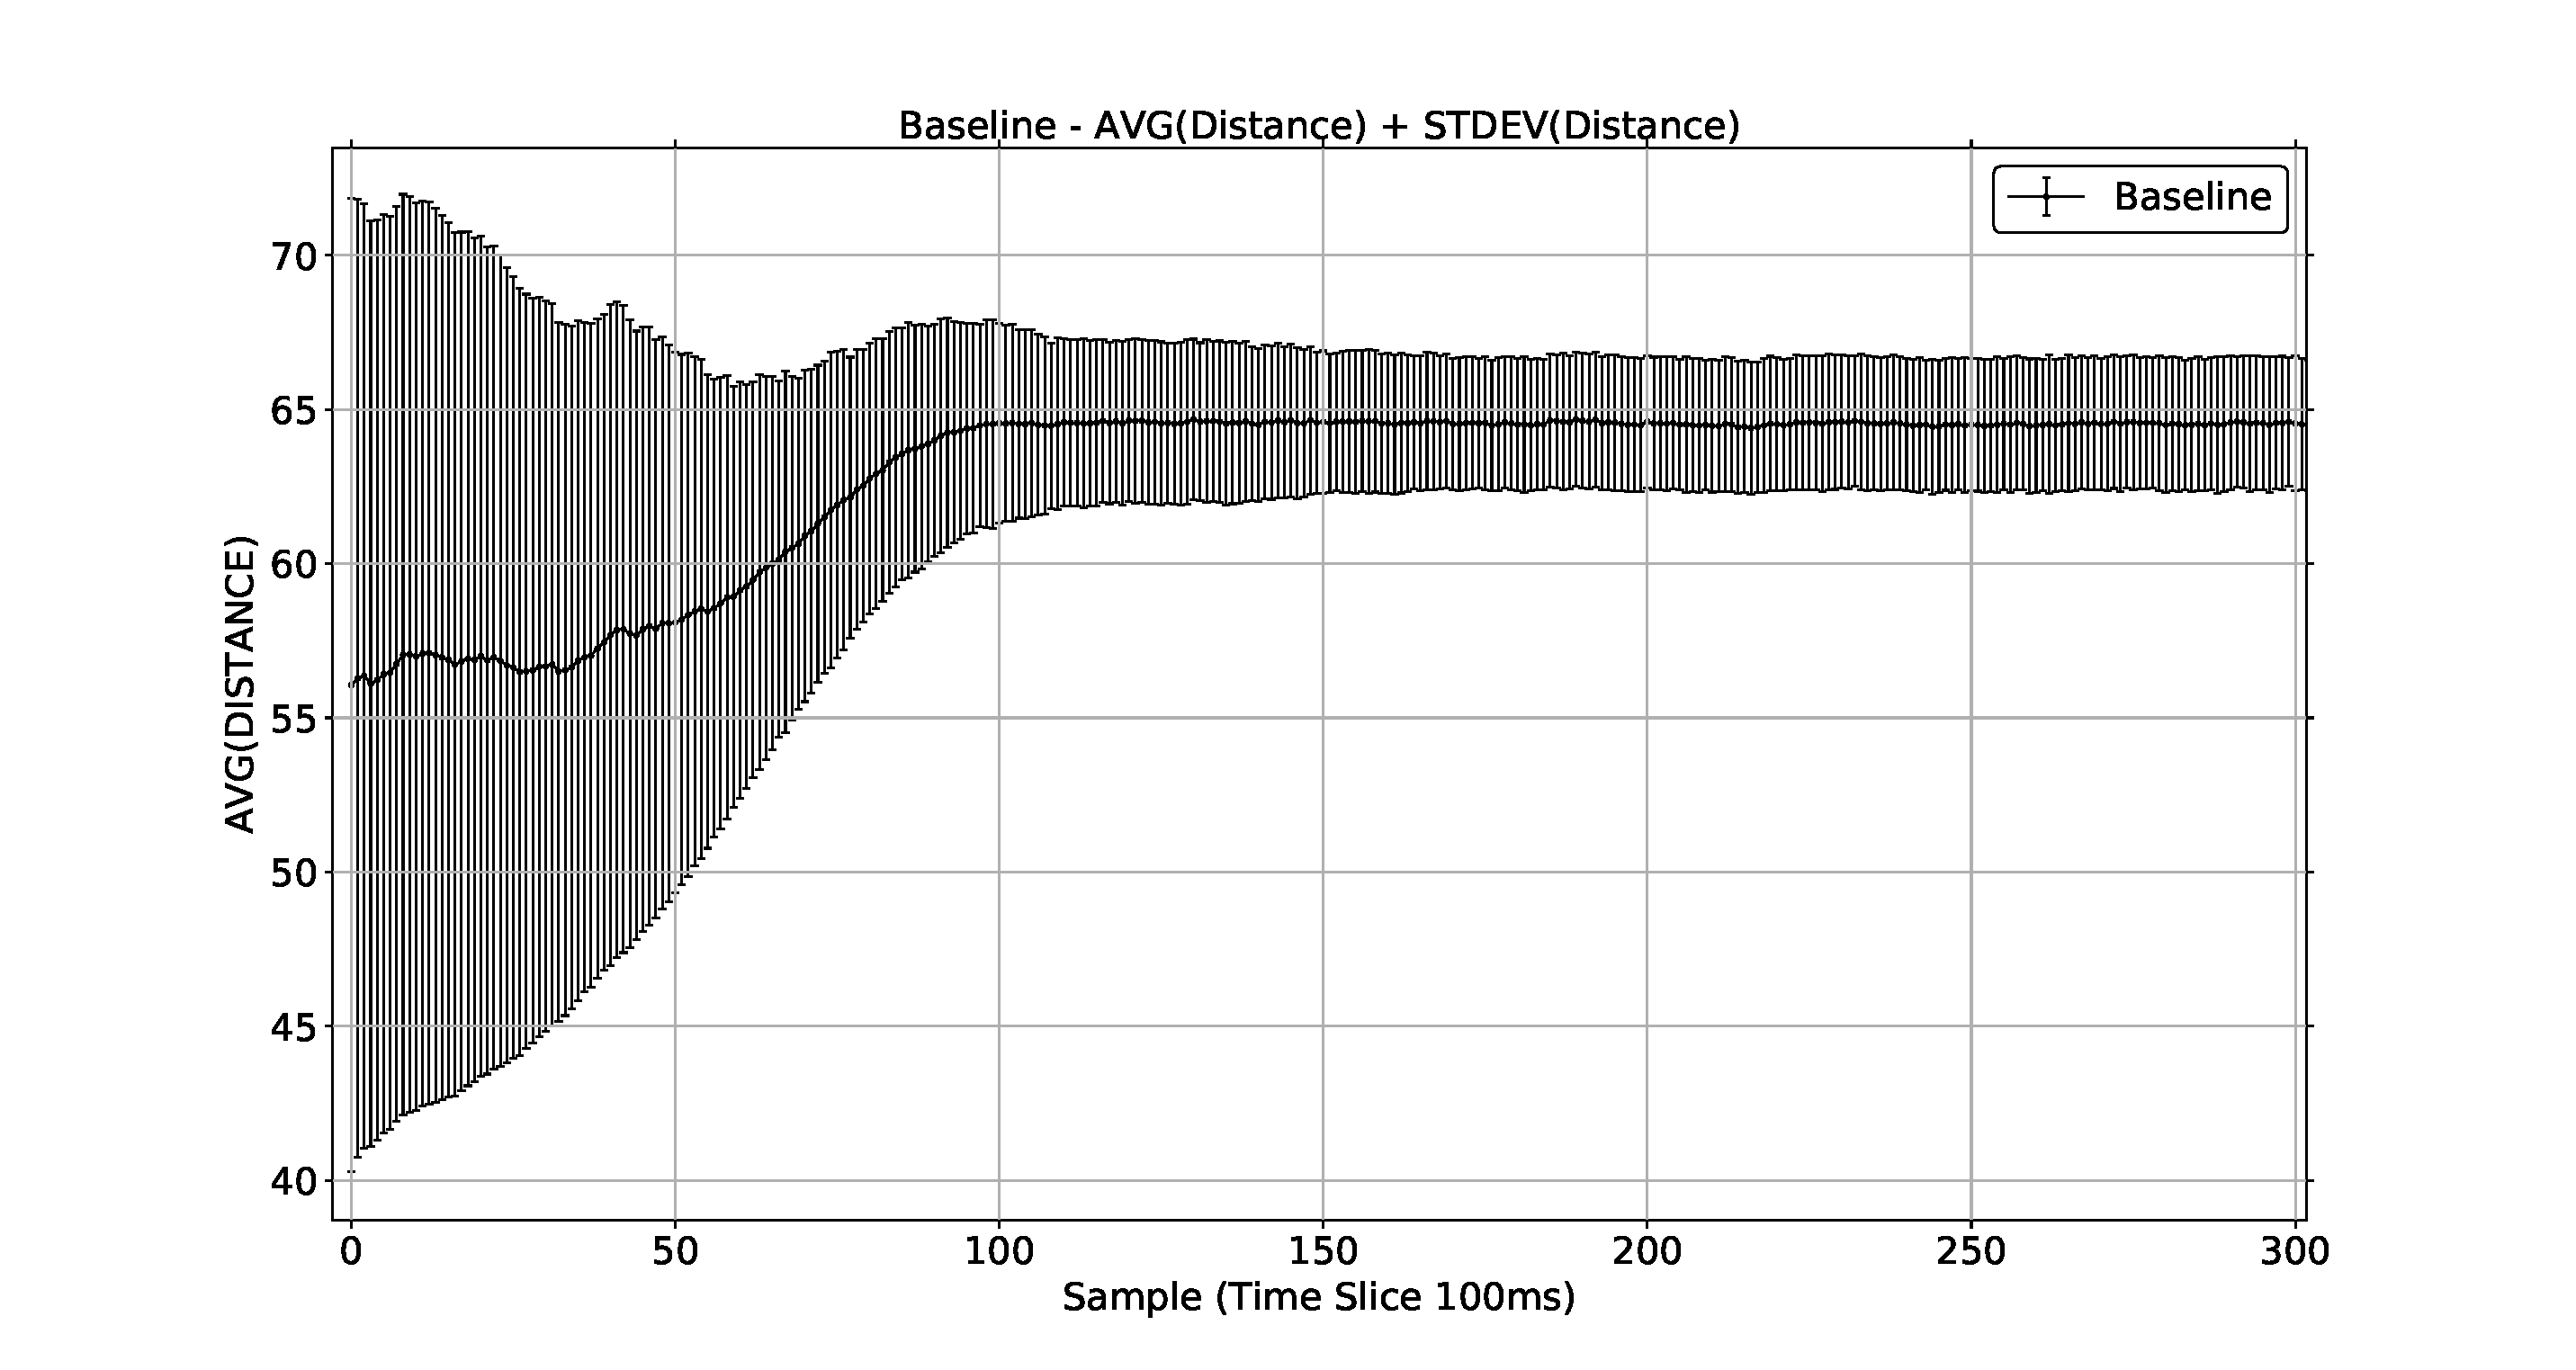
\includegraphics[width=9cm]{figures/BaselineDistance1}
\end{center}
\caption{Baseline internal movement - distance\label{coord:BaselineDistance1}}
\end{figure}

\section{Magnitude based metric\label{section:MagnitudeDynamics}}
Magnitude based internal movement (\textit{agent resultant magnitude}) is measured by identifying the balance between the repulsion and cohesion between agents. `Jitter' in the case of the \textit{agent resultant magnitude} metric is measured as the deviation of the magnitude lengths created by the agents. The identification of this deviation produces the clarifying part of the \textit{agent resultant magnitude} metric.
%% The magnitude based metric identifies the resultant internal magnitude (vector magnitude) through the cohesive and repulsive magnitudes that exist between each agent pair in a swarm. 
The \textit{agent resultant magnitude} is identified by Gazi and Passino~\cite{GP:11} and Barnes et al~\cite{BFV:07} as a `resultant characteristic' of a swarm. There are two ways of using the cohesion and repulsion in identifying a resultant vector. The two vectors can be added as absolute values to give an overall `size' to the magnitude that is affecting each relationship. Alternatively the resultant magnitude can be the sum of the actual magnitudes. The repulsion vector has a negative magnitude and the cohesion vector has a positive magnitude. In this paper the magnitude analysis will be based on summing the two vectors to determine the result of the inter-agent interaction, although both mechanisms could be used for a comparitive analysis. This paper will refer to the resultant magnitude as the \text{`agent resultant magnitude'} of the relationship. The `state' of a swarm is therefore the effect the environmental constraints and algorithms have upon the agent resultant magnitude. the \text{`agent resultant magnitude'} can be considered part of the `quality' measure for a swarm's performance.

If the \textit{agent resultant magnitude} is negative (absolute values would prevent this analysis) the swarm's bias is to expand as the repulsion is greater than cohesion. This is seen in the disorgansed stage of a swarm. The disorganised stage is the initial random deployment of the agents. If the \textit{agent resultant magnitude} is positive then the swarm is exhibiting a tendency to contract and this indicates the swarm is a cohesive entity. This could also be described as the swarm being `sticky' as the agents bias is to `pull' towards each other.

The \textit{agent resultant magnitude} on its own does not give a complete measure of a swarm's internal state. There needs to be a qualifying component to the metric  that identifies the degree of deviation in the resultant magnitude, this is the \textit{jitter}. The smaller the deviation the more uniform the structure of the swarm. These two components identify the degree to which a swarm has progressed towards a stable state.
 
The \textit{agent resultant magnitude} provides a view of the swarm's state through the balance between the repulsive and the cohesive vectors that are being applied to each agent. The deviation component identifies the degree to which the swarm has stabilised. The ideal status for inter-agent interactions would be for the agents to have a resultant vector (\textit{agent resultant magnitude}) of zero or above. This would indicate that the agents are distributed such that they are at their distribution limit (outer most range of the cohesion field) or at a level that causes the agents to `pull' together. The ideal degree of deviation is zero as this indicates an even distribution of agents. These two aspects of a swarm's features are not considered by Gazi and Passino~\cite{GP:11} or Barnes et al~\cite{BFV:07} as a means of quantifying the structure of a swarm in terms of stability.

\section{Magnitude based internal movement model}\label{Section:StabilityModel}
Using the formulae for the calculation of cohesion~(Equation \ref{eq:FlyToCentre1}) and repulsion~(Equation \ref{eq:Repulsion1}) for every agent and its neighbours it is possible to calculate an \textit{agent resultant magnitude} value (sum of agent resultant magnitudes). This value represents the overall `potential' of an agent. This magnitude when normalised produces a component of the \textit{movement-destination vector} for a swarm. If the agent resultant magnitude is zero (null vector) then the agent will not move. $P(b)$ is the \textit{inter-agent resultant magnitude vector} for agent $b$ defined by:

\begin{equation}
\label{eq:BotStabilityT}
P(b) = k_cv_c(b) + k_r v_r(b)
\end{equation}

Although it is possible for agent $b$ to have a resultant vector of null there could still be a variation in the constituent components. The variation calculation (standard deviation) is shown in~\ref{Section:VarianceInPotential}. \ref{eq:SwarmStabilityMetricT} is the mean of the \textit{agent resultant magnitudes} for an agent and its neighbours where $|nbr(b)|$ is the number of neighbours.

\begin{equation}
\label{eq:SwarmStabilityMetricT}
\mu_p(b) = \frac{P(b)}{|nbr(b)|}
\end{equation}

%% \ref{eq:SwarmStabilityMetricT} should be considered as being applied at discrete points in time within a simulation. The formulae could also be shown based on time $t$ (\ref{eq:SwarmStabilityMetricT2}) where $b_t$ is an agent at a specific time interval. All formulae for agent resultant magnitude in this thesis will be considered as being applied at a point in time and will therefore be shown without a $t$ subscript.
%% 
%% \begin{equation}
%% \label{eq:SwarmStabilityMetricT2}
%% \mu_p(b_{t}) = \frac{P(b_{t})}{|nbr(b_{t})|}
%% \end{equation}

To identify the swarm based \textit{agent resultant magnitude}~Equation~\ref{eq:SwarmStabilityMetricT} must be extended to iterate over all the agents in the swarm. \ref{eq:SwarmStabilityMetricT3} shows $\mu_p(S)$~as the swarm based magnitude.

\begin{equation}
\label{eq:SwarmStabilityMetricT3}
\mu_p(S) = \frac{\mathlarger{\sum_{b \in S} P(b)}}{\mathlarger{\sum_{b \in S}}|nbr(b)|}
\end{equation}

\section{Standard deviation in agent resultant magnitude metric}\label{Section:VarianceInPotential}
To improve the metric clarification in terms of the deviation from the \textit{agent resultant magnitude} norm is calculated. The standard deviation of the entire swarm  is shown in Equation \ref{eq:SwarmStabilityMetricT}.

The standard deviation is calculated as Equation~\ref{eq:SwarmStabilityQuotientT} where $\sigma_p(S)$ is the standard deviation at a time $t$ and $\mu_p(S)$ is the mean at the same point in time. 

\begin{equation}
\label{eq:SwarmStabilityQuotientT}
\sigma_p(S) = \sqrt{\frac{\mathlarger{\sum_{b \in S}}~\mathlarger{\sum_{b' \in nbr(b)}}\Big(P(b')-\mu_p(S)\Big)^2}{\mathlarger{\sum_{b \in S}}|nbr(b))|}}
\end{equation}

The metric for the internal movement is a set of numbers, the mean and standard deviation of the swarm's internal \textit{agent resultant magnitude} derived from each agent and its neighbour interactions~(Equation~\ref{eq:SwarmPotentialMagnitude}). The pair $\mu_p(S)$, $\sigma_p(S)$ may be written informally as: 

\begin{equation}
\label{eq:SwarmPotentialMagnitude}
\psi_p = \mu_p(S)\pm \sigma_p(S)
\end{equation}

\begin{figure}[H]
\begin{center}
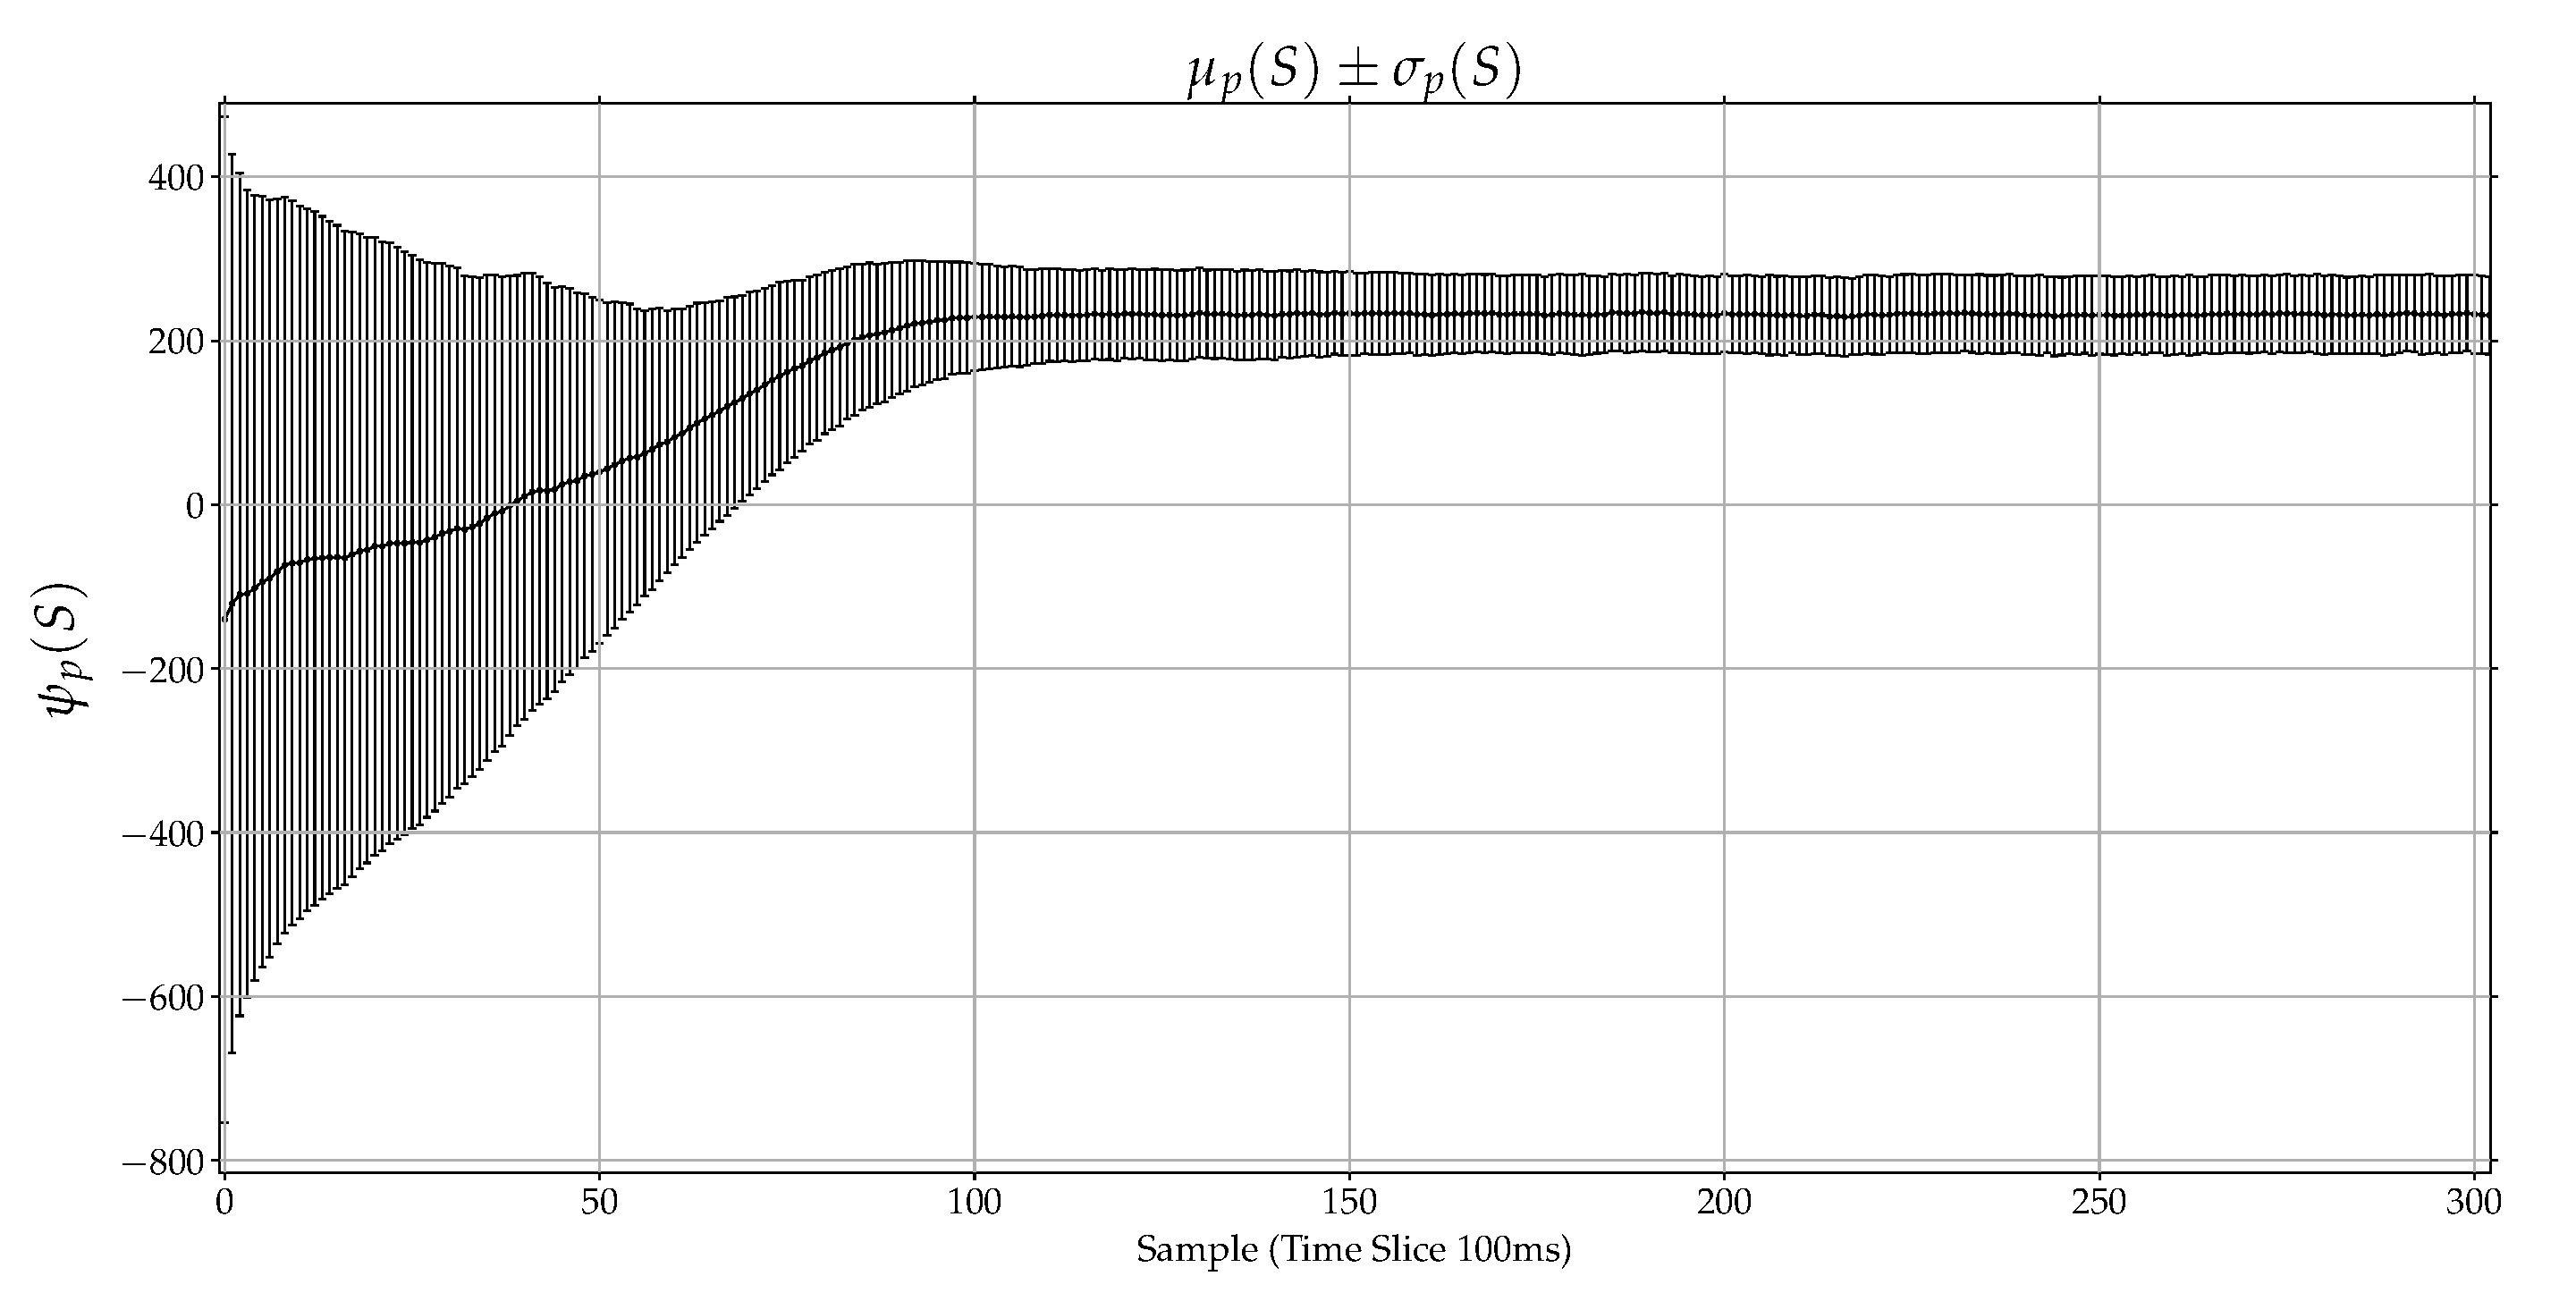
\includegraphics[width=9cm]{figures/BaselineMagnitude1}
\end{center}
\caption{Baseline internal movement - magnitude\label{coord:BaselineMagnitude1}}
\end{figure}

\section{Conclusion - metric comparison\label{metric:MagnitudeDistanceComparison}}
The two metrics appear to be similar in terms of the measurement of the structure of a swarm. The main difference is in how these two metrics can be used when examining the state of the swarm.

Both metrics identify the state of a swarm with respect to deviations in the dispersement of the agents from a mean. 

The main difference in the metrics is that the distance metric is based upon the physical \textit{distribution} of the agents and the magnitude based metric is based upon the logical \textit{interaction} of the agents.

The distance based metric provides and analysis of the actual distribution of the agents at a point in time and allows the agitation of the swarm to be assessed without considering the possible distribution of agents that the field effects \textit{could} produce.

The \textit{agent resultant magnitude} metric provides a view of the interaction magnitude. This provides an indication of the swarm's potential movement. This is independent of the physical distribution. The lack of dependence on the physical distribution allows the metric to be used in heterogeneous field effect swarms~\ref{additional:fieldsWork} where the physical distribution of agents may vary but due to the differing feild ranges the resultant magnitudes balance. 

Combining the two metrics allows a deeper evaluation of a swarm to be made. Consider the following: the repulsion field is increased but the internal distances do not change as a result the \textit{agent resultant magnitude} rises: This indicates `something' is confining the swarm's distribution. This analysis could be used in identifying effective swarm distribution for the coverage of a sensor array as discussed by Ramaithitima et al.~\cite{RWBK:15}

\begin{figure}[H]
\begin{center}
\includegraphics[width=8cm]{figures/FieldEffects2}
\end{center}
\caption{Complex swarm interactions\label{additional:fieldsWork}}
\end{figure}

\bibliographystyle{plain}
\bibliography{thesis}

\end{document}
